%\documentclass[wcp,gray]{jmlr}
\documentclass[wcp]{jmlr}

\usepackage{booktabs}
\usepackage{graphicx}
\usepackage{amsmath,amssymb}
\usepackage{hyperref}
\usepackage{lineno}

\pagenumbering{gobble}
\newcommand{\cs}[1]{\texttt{\char`\\#1}}
\makeatletter
\let\Ginclude@graphics\@org@Ginclude@graphics
\makeatother

\jmlryear{2026}
\jmlrworkshop{ACML 2026}

\title[Bayesian Fusion for Multi-Sensor Damage Assessment]{Bayesian Uncertainty Fusion for Multi-Sensor Remote Sensing
Damage Assessment:\\A Case Study of Sentinel-2 and VIIRS in Mariupol}

\author{
  \Name{Author Name} \Email{author@university.edu}\\
  \addr{Department of Statistics, University Name}
}

\editors{}

\begin{document}

\makeatletter
\let \@jmlrpages \@empty
\makeatother

\maketitle

% =====================================================================
\begin{abstract}
Multi-sensor fusion for damage assessment typically assumes that different
sensors observe the same latent damage state. This assumption fails when
sensors capture distinct physical dimensions of damage. We fuse
Sentinel-2 (S2) spectral indices and VIIRS nighttime light (NTL) loss to
estimate war-related damage in Mariupol, Ukraine, and find systematic
disagreement between the two signals: S2 primarily captures surface
alteration (structural damage), while VIIRS registers functional cessation
through reduced nighttime illumination. Under a Bayesian hierarchical model
with a single latent damage state, the posterior collapses to a
near-uniform spatial estimate ($p_i \in [0.151, 0.157]$), losing
essentially all grid-level differentiation (KL divergence vs.\ global mean
$\approx 0$ nats). Kullback-Leibler and Jensen-Shannon divergence analysis
quantifies a fusion suppression ratio of $46.8\%$, demonstrating that
nearly half of the best single-sensor information is suppressed under the
joint model. Dempster-Shafer evidence theory preserves conflict through
belief/plausibility intervals (Belief~$=0.145$, Plausibility~$=0.369$).
Grid-level comparison reveals $49.9\%$ genuine agreement, $10.2\%$
uncertainty-compatible, and $28.1\%$ divergence between the two fusion
paradigms. Under the UNOSAT validation setting, VIIRS shows stronger
agreement with reference labels (AUC~$=0.829$) than the current S2-derived
index (AUC~$=0.332$). We conclude that adding sensors does not
automatically improve damage estimation: multi-sensor fusion benefits
inference only when sensors measure compatible damage dimensions or when
the model explicitly accommodates multiple latent states.
\end{abstract}

\begin{keywords}
Bayesian hierarchical model; Dempster-Shafer evidence theory;
Kullback-Leibler divergence; multi-sensor fusion; damage assessment;
Sentinel-2; VIIRS
\end{keywords}

% =====================================================================
\section{Introduction}\label{sec:intro}

Rapid damage assessment following armed conflicts and natural disasters is
critical for humanitarian response and reconstruction planning. Satellite
remote sensing offers a scalable, repeatable means of surveying affected
areas where ground access is limited or unsafe. Optical sensors such as
Sentinel-2 (S2) detect surface changes through pre- and post-event spectral
comparison, while low-light imagers such as the VIIRS Day-Night Band (DNB)
capture reductions in nighttime illumination associated with infrastructure
destruction, power outages, and population displacement
\cite{zhang2023,xiao2024}.

Multi-sensor fusion is commonly motivated by the assumption that combining
multiple data sources improves estimation accuracy by reducing measurement
noise. This reasoning holds when sensors provide redundant observations of
the \emph{same} latent quantity. However, when different sensors respond to
different physical manifestations of damage---structural alteration versus
functional loss---forcing them into a single latent state may produce
counterintuitive behavior, including posterior collapse and loss of spatial
differentiation.

We investigate this problem through a case study of Mariupol, Ukraine,
which experienced extensive damage during the 2022 Russia-Ukraine conflict.
We construct S2 spectral damage indices and VIIRS NTL loss indicators at a
500~m grid resolution, validate against UNOSAT external reference labels,
and apply three complementary analytical frameworks: Bayesian hierarchical
modeling, KLD/JSD information analysis, and Dempster-Shafer (D-S) evidence
theory. Our study addresses three specific questions:

\begin{enumerate}
  \item How do S2 and VIIRS each align with UNOSAT external reference
    labels under this validation setting?
  \item How does a Bayesian hierarchical model behave when fusing two
    sensors that systematically disagree?
  \item Does adding a second sensor improve information gain, or can
    sensor conflict suppress usable information?
\end{enumerate}

The principal contributions are: (1)~a Bayesian hierarchical uncertainty
framework for fusing S2 and VIIRS damage probabilities without requiring
ground-truth labels; (2)~a quantitative decomposition of single-sensor
information, fused information, and inter-sensor conflict using KLD and
JSD; and (3)~a grid-level comparison of Bayesian point-estimate fusion with
D-S interval-based evidence combination under conflicting evidence.

% =====================================================================
\section{Study Area and Data}\label{sec:data}

\subsection{Mariupol Area of Interest}

The study area covers Mariupol and surroundings in southeastern Ukraine
(37.42\textdegree{}E--37.72\textdegree{}E, 47.05\textdegree{}N--47.18\textdegree{}N),
a region that experienced extensive structural and functional damage during
the 2022 conflict. The AOI spans approximately 23~km east-west by 14~km
north-south and is divided into 1{,}380 grid cells at 500~m resolution.

\subsection{Sentinel-2 Imagery}

Sentinel-2 Level-2A surface reflectance products were acquired for
pre-event (2021-05-23) and post-event (2022-05-08) dates, covering tiles
T37TCN and T37TDN. The pre-event date was chosen to match the same
phenological period one year prior to minimize seasonal vegetation effects.
Spectral indices (NDVI, NBR, and soil-adjusted variants) were computed from
10~m and 20~m bands and aggregated to 500~m grid cells. Per-index delta
(post minus pre) was normalized by the spatial standard deviation of the
pre-event index, and the final S2 damage score $p_{\text{S2}}$ was obtained
by averaging z-scores across indices and transforming to $[0,1]$.

\subsection{VIIRS Nighttime Light Data}

VIIRS DNB monthly composite data (VNP46A3) were obtained for matching pre-
and post-event periods. DNB radiance values were filtered using the
mandatory quality flag. Per-grid mean NTL radiance and the relative NTL
loss rate $R_i = (L_{\text{pre},i} - L_{\text{post},i})/L_{\text{pre},i}$
were computed at 500~m resolution and transformed to a damage probability
$p_{\text{VIIRS}}$ via sigmoid calibration.

\subsection{UNOSAT External Reference Labels}

UNOSAT damage assessment data for the Livoberezhnyi District of Mariupol
(dated 12 May 2022), produced through visual interpretation of
very-high-resolution satellite imagery, were used as an external reference.
Building footprints with damage classifications were spatially joined to
the 500~m grid. A strict matching protocol was applied: Main\_Dam\_1~$=14$
(destroyed) was treated as the positive class and Main\_Dam\_1~$=6$ (no
visible damage) as the negative class, yielding 995 labeled grids (32.8\%
positive). We emphasize that UNOSAT is an external reference rather than
absolute ground truth; it captures visually identifiable structural damage
but may miss functional damage or sub-detection-threshold structural
alteration.

\begin{table}[htp]
\centering
\caption{Data sources and preprocessing summary.}
\label{tab:data}
\begin{tabular}{@{}lllll@{}}
\toprule
\textbf{Source} & \textbf{Product} & \textbf{Pre-Date} & \textbf{Post-Date} & \textbf{Resolution} \\
\midrule
Sentinel-2 MSI  & L2A Surface Reflectance  & 2021-05-23 & 2022-05-08 & 10--20~m (500~m grid) \\
VIIRS DNB       & VNP46A3 Monthly Composite & 2021-05    & 2022-05    & 500~m native \\
UNOSAT          & Visual Damage Assessment  & ---        & 2022-05-12 & Building-level \\
\midrule
\textbf{Grid}   & \textbf{Cells} & \textbf{CRS} & \textbf{Valid S2} & \textbf{Valid VIIRS} \\
500~m fishnet   & 1{,}380        & WGS84        & 1{,}131 (82.0\%)   & 1{,}268 (91.9\%) \\
\bottomrule
\end{tabular}
\end{table}

% =====================================================================
\section{Methods}\label{sec:methods}

\subsection{Sentinel-2 Spectral Damage Index}

For each 500~m grid cell, spectral indices are computed from all valid
10~m and 20~m pixels within the cell for both pre- and post-event images.
The per-index change $\Delta_k$ is normalized by the pre-event spatial
standard deviation $\sigma_k$ to produce a z-score. The S2 damage
probability is the logistic transform of the mean z-score, clipped to
$[10^{-4}, 1-10^{-4}]$. Grids with fewer than 20\% valid S2 pixels
are marked as missing.

\subsection{VIIRS Nightlight-Loss Index}

The VIIRS damage probability $p_{\text{VIIRS},i}$ is derived from the
relative NTL loss rate. Negative loss rates (grids that became brighter)
are clamped to zero. The raw loss rate is transformed via a sigmoid
function calibrated on the empirical distribution of loss rates across
the AOI. Grids with fewer than 10 valid DNB observations in either
period are marked as missing.

\subsection{UNOSAT External Validation}

Each damage score is evaluated as a binary classifier against the UNOSAT
strict label set. Metrics reported include area under the ROC curve (AUC),
area under the precision-recall curve (PR-AUC), Brier score, and Spearman
rank correlation. Validation is performed for raw S2, raw VIIRS,
logit-averaged fusion, and D-S belief, plausibility, and midpoint.

\subsection{Bayesian Hierarchical Uncertainty Fusion}\label{sec:bayes}

We specify a three-level logit-normal hierarchical model with a single
latent damage state. Let $y_{ik} = \text{logit}(p_{ik})$ for sensor
$k \in \{\text{S2}, \text{VIIRS}\}$ at grid $i$. The model is:

\begin{align}
\text{Level 1:}\quad
  y_{i,\text{S2}} &\sim \mathcal{N}(\theta_i + \delta_{\text{S2}},\;
                     \sigma_{\text{S2}}^2) \label{eq:L1s2}\\
  y_{i,\text{VIIRS}} &\sim \mathcal{N}(\theta_i,\;
                         \sigma_{\text{VIIRS}}^2) \label{eq:L1v}\\
\text{Level 2:}\quad
  \theta_i &= \text{logit}(p_i) = \mu + \eta_i,\quad
  \eta_i \sim \mathcal{N}(0, \tau^2) \label{eq:L2}\\
\text{Level 3:}\quad
  \mu &\sim \mathcal{N}(0, 2^2),\quad
  \tau \sim \text{HalfCauchy}(1),\quad
  \sigma_k \sim \text{HalfCauchy}(0.5) \label{eq:L3}
\end{align}

The bias term $\delta_{\text{S2}}$ captures the S2 sensor's systematic
offset relative to the latent state. Posterior inference uses the
No-U-Turn Sampler (NUTS) with 4 chains of 1{,}000 tuning and 1{,}000
sampling iterations. Single-sensor baseline models are fitted independently
by setting the unused sensor's likelihood term to zero.

\subsection{KLD/JSD Information Gain Analysis}\label{sec:kld}

We quantify single-sensor and fused information using Bernoulli-level
Kullback-Leibler divergence. For two Bernoulli distributions parameterized
by $p$ and $q$:

\begin{equation}
\mathrm{KL}(p \,\|\, q) = p\log\frac{p}{q} + (1-p)\log\frac{1-p}{1-q}
\label{eq:kl}
\end{equation}

\begin{equation}
\mathrm{JSD}(p, q) = \tfrac{1}{2}\mathrm{KL}(p \,\|\, m)
  + \tfrac{1}{2}\mathrm{KL}(q \,\|\, m),\quad
  m = \tfrac{1}{2}(p+q)
\label{eq:jsd}
\end{equation}

All divergences use natural logarithms (units: nats). Probabilities are
clipped to $[10^{-9}, 1-10^{-9}]$ for numerical stability. We compute three
families of metrics: (1)~single-sensor information gain against a neutral
prior $p=0.5$; (2)~spatial differentiation against each model's global
mean; and (3)~fusion suppression, defined as
$\text{suppression} = (\max\text{KL} - \text{KL}_{\text{both}}) /
\max\text{KL}$. Sensor conflict is measured by JSD between the S2-only and
VIIRS-only posteriors.

\subsection{Dempster-Shafer Evidence Fusion and Consistency
Comparison}\label{sec:ds}

Basic probability assignments (BPAs) are constructed for three states:
Damage ($D$), No Damage ($N$), and Uncertainty ($U$). For sensor $k$,
$m_k(D) = \alpha_k \cdot p_k$, $m_k(N) = \alpha_k \cdot (1-p_k)$, and
$m_k(U)=1-\alpha_k$, where $\alpha_k$ is derived from the sensor's valid
observation ratio. Dempster's rule combines the BPAs to yield joint belief
and plausibility:
$\text{Bel}(D) = m_{12}(D)/(1-K)$,
$\text{Pl}(D) = (m_{12}(D)+m_{12}(U))/(1-K)$,
where $K$ is the conflict coefficient.

Grid-level consistency between Bayesian and D-S estimates is classified
using four rules: \emph{strong consistent} if the Bayesian posterior mean
falls within $[\text{Bel}(D), \text{Pl}(D)]$ and the D-S interval is
narrow (below the 75th percentile of interval width); \emph{uncertainty-compatible}
if the Bayesian mean falls within a wide D-S interval; \emph{weak consistent}
if the Bayesian 95\% CI overlaps the D-S interval but the mean is outside;
and \emph{divergent} if the Bayesian CI lies entirely above or below the
D-S interval.

% =====================================================================
\section{Results}\label{sec:results}

\subsection{S2 and VIIRS Provide Non-Equivalent Damage Signals}\label{sec:res-disagree}

\begin{figure}[htp]
\begin{center}
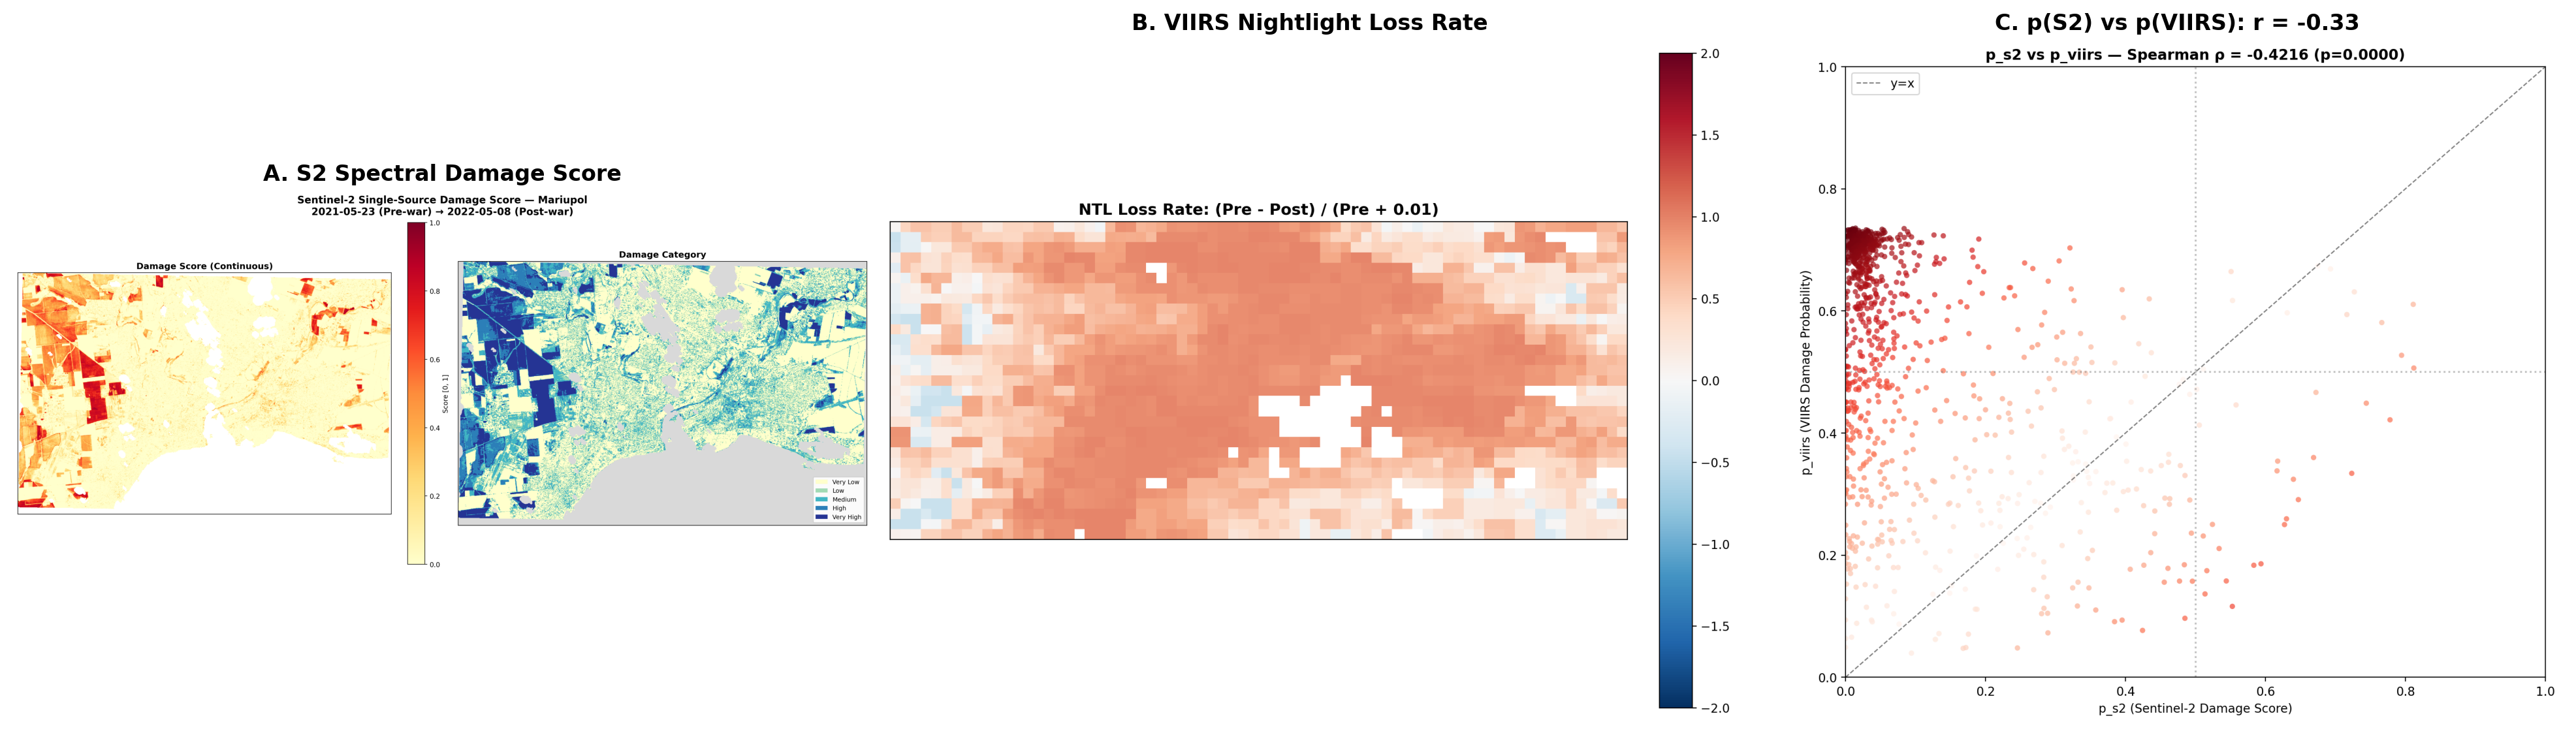
\includegraphics[width=0.95\textwidth]{figures/fig1_sensor_disagreement.png}
\caption{\textbf{S2 and VIIRS capture distinct damage dimensions.}
(A)~The S2 spectral damage score highlights urban-core surface alteration.
(B)~The VIIRS NTL loss rate shows a more diffuse spatial pattern extending
into peri-urban areas. (C)~The scatter plot reveals a negative correlation
($r = -0.33$) between the two scores: grids with high S2 damage do not
systematically correspond to grids with high VIIRS damage, and vice versa.
This indicates that S2 and VIIRS are not redundant observations of a single
latent damage state.}
\label{fig:disagree}
\end{center}
\end{figure}

Figure~\ref{fig:disagree} establishes the foundational observation of this
study. The S2 damage score (Panel~A) concentrates elevated values in the
urban core and industrial zones, consistent with the spectral signature of
exposed rubble, disturbed soil, and altered vegetation---manifestations of
physical structural damage. The VIIRS NTL loss rate (Panel~B) shows a more
diffuse spatial pattern: while urban areas exhibit NTL reduction, elevated
loss rates also appear in peri-urban and suburban zones, consistent with
widespread power outages and population displacement that extend beyond the
footprint of direct structural destruction.

The scatter plot (Panel~C) quantifies the disagreement: the Pearson
correlation between $p_{\text{S2}}$ and $p_{\text{VIIRS}}$ is $r = -0.33$.
Grids form two distinct clusters---one where S2 indicates high damage but
VIIRS does not (lower-right: structural damage with retained nightlight),
and another where VIIRS indicates high damage but S2 does not (upper-left:
functional loss without visible structural change). These are not
measurement errors but genuine physical phenomena: a structurally intact
but unlit building (power outage) and a demolished building near a
functioning streetlight produce opposite sensor signatures.

\subsection{UNOSAT Validation Under This Reference Setting}\label{sec:res-unosat}

\begin{figure}[htp]
\begin{center}
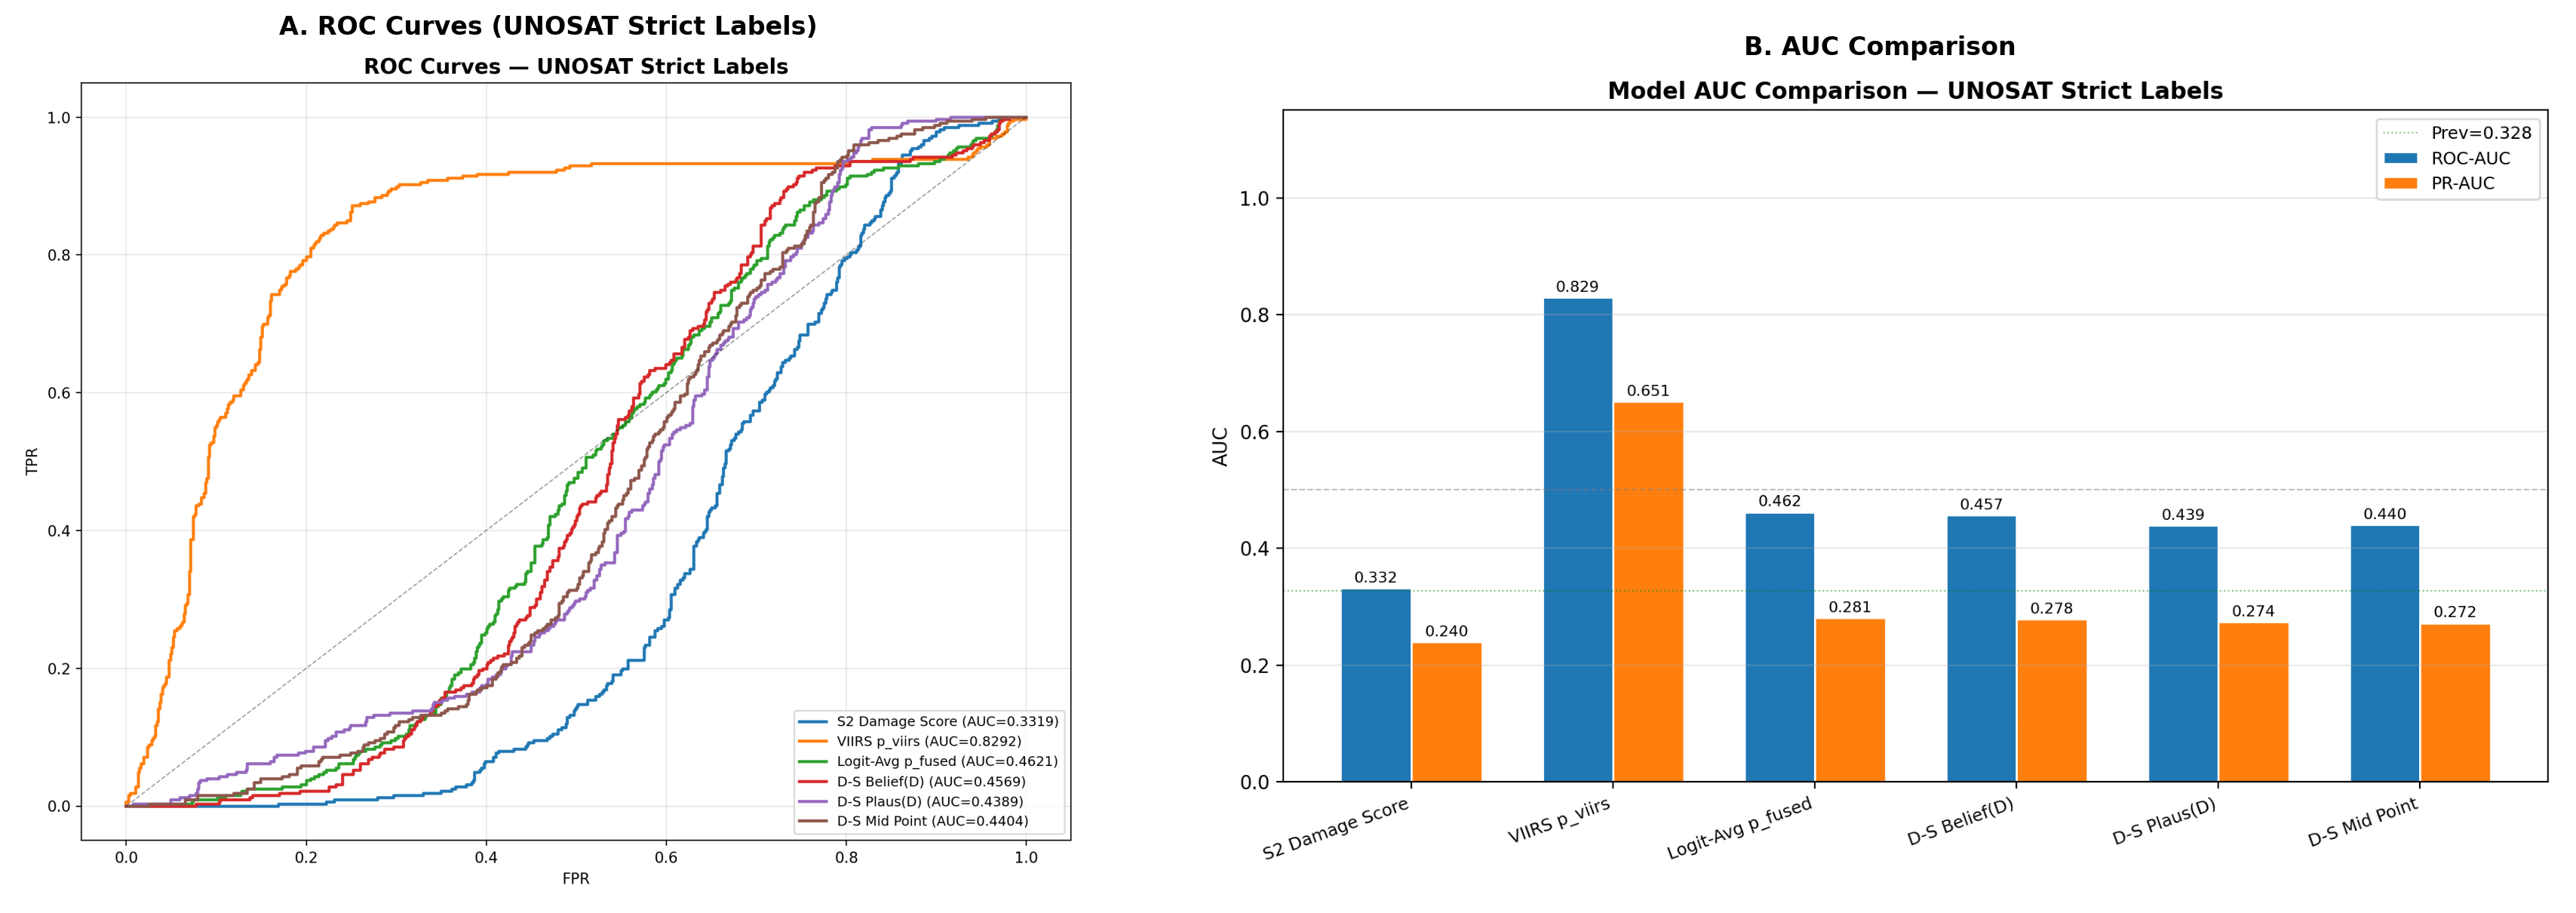
\includegraphics[width=0.95\textwidth]{figures/fig2_unosat_validation.png}
\caption{\textbf{UNOSAT external validation.}
(A)~ROC curves against UNOSAT strict labels ($n=995$, $32.8\%$ positive).
VIIRS achieves AUC~$=0.829$ (Spearman $r=0.535$, Brier~$=0.222$). The
current S2-derived index yields AUC~$=0.332$, below the random baseline.
All fusion-based scores---logit-average (AUC~$=0.462$), D-S belief
(AUC~$=0.457$), plausibility (AUC~$=0.439$), and midpoint
(AUC~$=0.440$)---perform below VIIRS alone. (B)~AUC barplot comparison:
adding S2 to VIIRS degrades discriminative performance under every
aggregation method tested.}
\label{fig:unosat}
\end{center}
\end{figure}

Figure~\ref{fig:unosat} presents the external validation benchmark. Three
patterns emerge. First, VIIRS shows stronger agreement with the UNOSAT
reference labels under this validation setting (AUC~$=0.829$, Spearman
$r=0.535$), while the current S2-derived index is weakly aligned
(AUC~$=0.332$, $r=-0.274$) and performs below the random-classifier
baseline. The S2 ROC curve lies predominantly below the diagonal, and its
PR curve is nearly flat at the prevalence baseline ($0.328$).

Second, all fusion-based scores perform below VIIRS alone: logit-averaged
fusion (AUC~$=0.462$), D-S belief (AUC~$=0.457$), D-S plausibility
(AUC~$=0.439$), and D-S midpoint (AUC~$=0.440$). This degradation is
consistent with the negative correlation observed in
Figure~\ref{fig:disagree}: combining a weakly aligned signal with a
well-aligned one introduces noise rather than complementary information
under single-score aggregation.

Third, the absolute performance ceiling is moderate: the maximum F1 score
is $0.630$ (VIIRS, at threshold~$=0.66$). This is expected given that
UNOSAT labels a specific subset of damage (visible structural damage to
buildings), while both S2 and VIIRS register signals extending beyond this
narrow definition. The validation thus benchmarks \emph{relative alignment}
rather than absolute accuracy.

\subsection{Bayesian Hierarchical Fusion Collapses Under the Single Latent
State Assumption}\label{sec:res-bayes}

\begin{table}[htp]
\centering
\caption{Bayesian hyperparameter posterior estimates. All parameters
converged with $\hat{R} < 1.01$ and 1 divergence in 4{,}000 draws.}
\label{tab:bayes_params}
\begin{tabular}{@{}lrrrrr@{}}
\toprule
\textbf{Parameter} & \textbf{Mean} & \textbf{SD} & \textbf{2.5\%} & \textbf{97.5\%} & \textbf{$\hat{R}$} \\
\midrule
$\mu$ (population mean, logit)        & $-1.695$ & $0.042$ & $-1.781$ & $-1.613$ & $1.000$ \\
$\tau$ (between-grid heterogeneity)   & $ 0.063$ & $0.047$ & $ 0.004$ & $ 0.172$ & $1.000$ \\
$\sigma_{\text{S2}}$ (S2 noise)       & $ 2.685$ & $0.059$ & $ 2.575$ & $ 2.803$ & $1.000$ \\
$\sigma_{\text{VIIRS}}$ (VIIRS noise) & $ 0.904$ & $0.018$ & $ 0.869$ & $ 0.940$ & $1.000$ \\
$\delta_{\text{S2}}$ (S2 bias)        & $-1.705$ & $0.042$ & $-1.789$ & $-1.624$ & $1.000$ \\
\bottomrule
\end{tabular}
\end{table}

\begin{figure}[htp]
\begin{center}
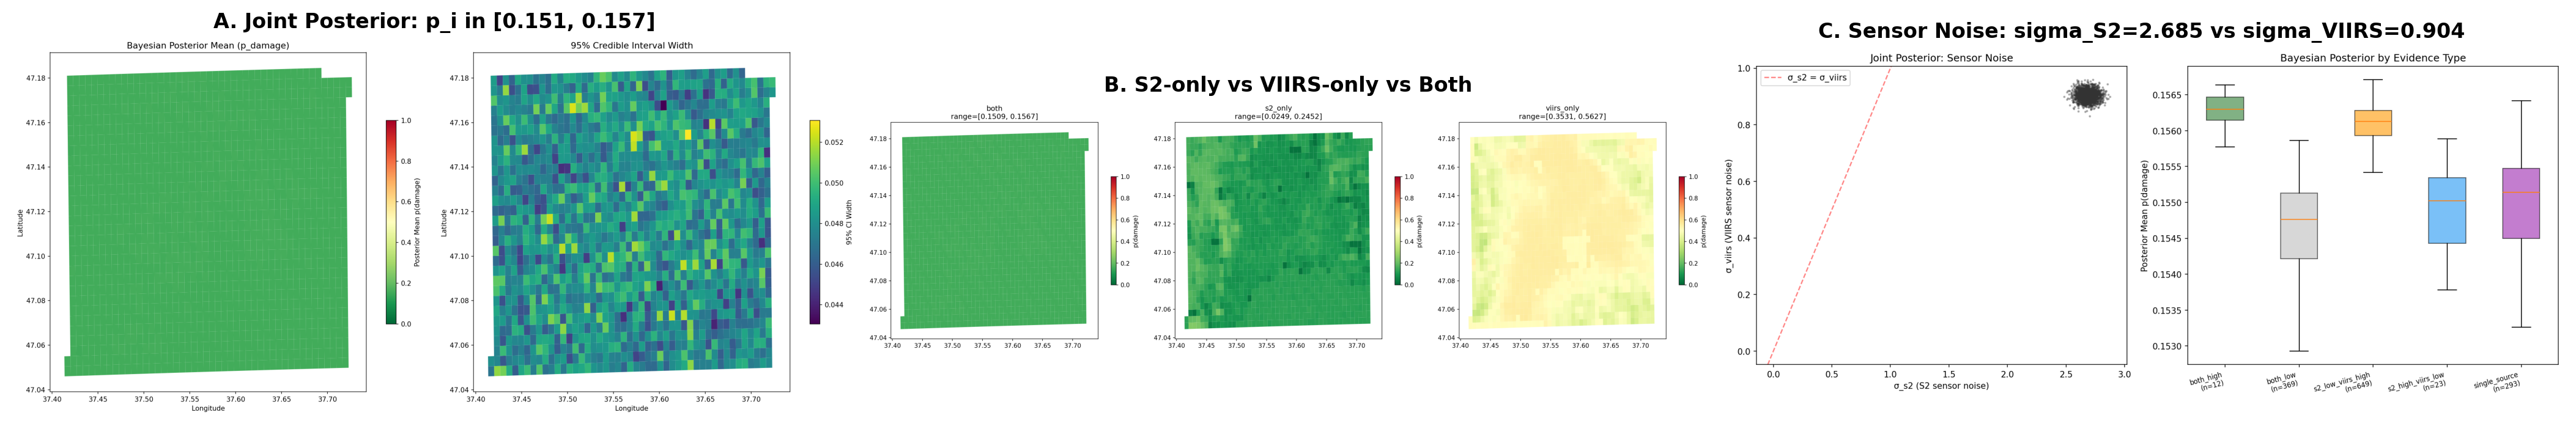
\includegraphics[width=0.95\textwidth]{figures/fig3_bayesian_collapse.png}
\caption{\textbf{Bayesian posterior collapse under single latent state
assumption.}
(A)~Joint posterior mean map: $p_i \in [0.151, 0.157]$, spatially
near-uniform. (B)~Sensor-only comparison: the S2-only posterior spans
$[0.025, 0.245]$ (22 pp range); the VIIRS-only posterior spans
$[0.353, 0.563]$ (21 pp range); the joint model collapses both into a
narrow band (0.006 pp range). (C)~Sensor noise estimates: the model learns
$\sigma_{\text{S2}} = 2.685$, approximately $3\times$ larger than
$\sigma_{\text{VIIRS}} = 0.904$ on the logit scale.}
\label{fig:bayes}
\end{center}
\end{figure}

Table~\ref{tab:bayes_params} and Figure~\ref{fig:bayes} present the
Bayesian hierarchical model results. Three parameter estimates jointly
explain the posterior collapse. First, $\tau = 0.063$ (95\% CI: $[0.004,
0.172]$) indicates that the joint data provide essentially no support for
shared grid-level heterogeneity after accounting for sensor bias and noise.
This is the formal statistical expression of the claim that S2 and VIIRS
cannot be reconciled into a single latent damage state: if they could,
$\tau$ would be substantially larger, reflecting genuine between-grid
variation in the common damage probability.

Second, $\sigma_{\text{S2}} = 2.685$ is approximately $3\times$ larger
than $\sigma_{\text{VIIRS}} = 0.904$ on the logit scale. The model thus
learns that S2 observations are substantially less precise, and the noisier
sensor receives commensurately less weight in determining the latent state.
Third, $\delta_{\text{S2}} = -1.705$ captures the directional nature of the
disagreement: S2 systematically reports damage probabilities approximately
$1.7$ logit units below the latent state.

Figure~\ref{fig:bayes}A makes the practical consequence visually stark: the
joint posterior mean is a near-uniform field of $p_i \approx 0.155$ across
all 1{,}380 grids. This map cannot distinguish a destroyed city block from
an intact agricultural field. Figure~\ref{fig:bayes}B reveals that this
collapse is an artifact of fusion, not of data poverty. The S2-only
posterior (top) and VIIRS-only posterior (bottom) each retain meaningful
spatial structure with 21--22 percentage point ranges. The joint model
(bottom of Panel~B) collapses both into a spatially invariant value.
Single-sensor MCMC diagnostics were weaker than the joint model (S2-only:
263 divergences, $\hat{R}_{\max}=1.21$; VIIRS-only: 122 divergences,
$\hat{R}_{\max}=1.35$), so single-sensor ranges should be interpreted as
diagnostic comparisons.

\subsection{KLD/JSD Shows Information Conflict Rather Than Information
Absence}\label{sec:res-kld}

\begin{table}[htp]
\centering
\caption{KLD/JSD information gain summary. All metrics in nats, computed
at the Bernoulli probability level with neutral prior $p=0.5$.}
\label{tab:kld}
\begin{tabular}{@{}lrrrr@{}}
\toprule
\textbf{Metric} & \textbf{Mean} & \textbf{Median} & \textbf{Min} & \textbf{Max} \\
\midrule
KL(S2 $\|$ neutral)          & 0.496 & 0.501 & 0.301 & 0.591 \\
KL(VIIRS $\|$ neutral)       & 0.007 & 0.006 & 0.000 & 0.072 \\
KL(Both $\|$ neutral)        & 0.261 & 0.261 & 0.259 & 0.269 \\
KL(S2 $\|$ S2$_{\text{global}}$)    & 0.003 & 0.001 & 0.000 & 0.050 \\
KL(VIIRS $\|$ VIIRS$_{\text{global}}$) & 0.007 & 0.005 & 0.000 & 0.075 \\
$\mathbf{KL(Both \| Both_{\text{global}})}$ & $\mathbf{\approx 0}$ & $\mathbf{\approx 0}$ & $\mathbf{\approx 0}$ & $\mathbf{<0.001}$ \\
JSD(S2, VIIRS)               & 0.146 & 0.150 & 0.053 & 0.212 \\
Fusion KL loss               & 0.235 & 0.240 & 0.041 & 0.329 \\
Fusion suppression ratio     & 0.468 & 0.479 & 0.137 & 0.557 \\
\bottomrule
\end{tabular}
\end{table}

\begin{figure}[htp]
\begin{center}
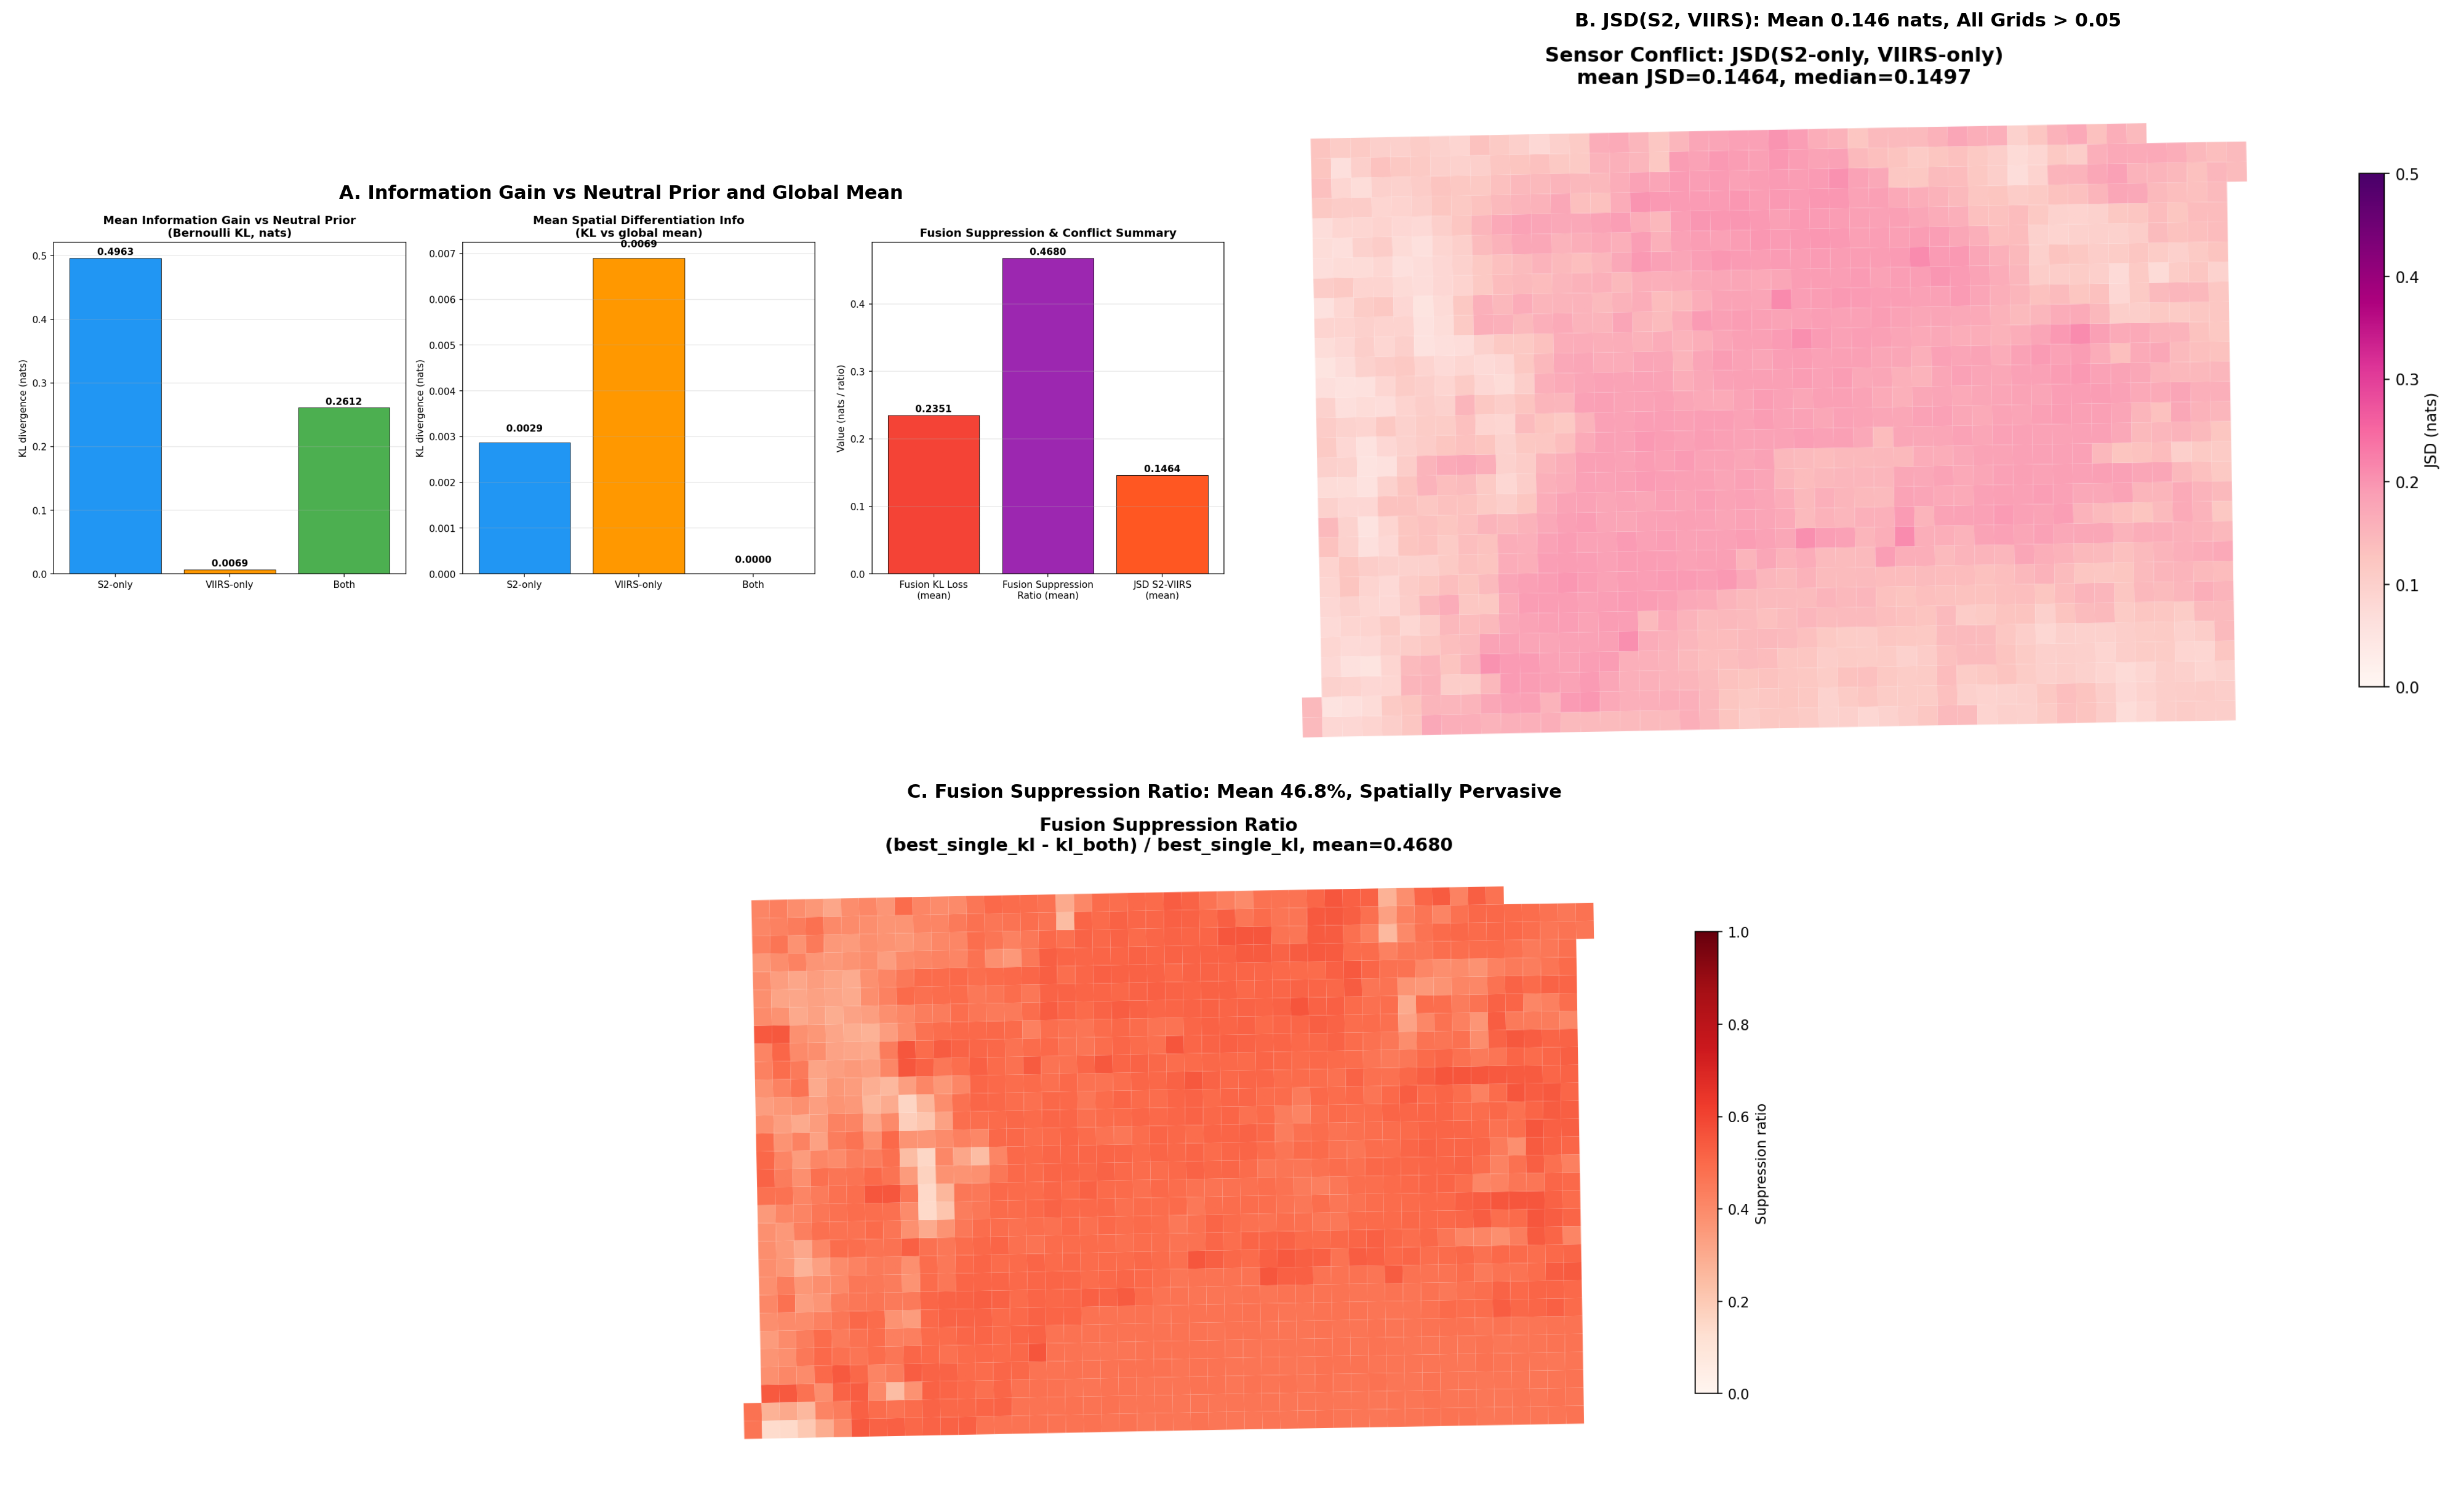
\includegraphics[width=0.95\textwidth]{figures/fig4_information_conflict.png}
\caption{\textbf{Information conflict, not information absence.}
(A)~KLD summary: S2 deviates strongly from the neutral prior ($p=0.05$
vs.\ $p=0.5$, KL~$=0.496$ nats); VIIRS remains near neutral (KL~$=0.007$
nats); the fused posterior falls in between (KL~$=0.261$ nats). Spatial
differentiation (KL vs.\ global mean, gray bars) is near zero for the fused
model. (B)~JSD conflict map: every grid has JSD(S2, VIIRS) $>0.05$ nats
(mean $0.146$, range $[0.053, 0.212]$). (C)~Fusion suppression map: the
fraction of the best single-sensor information lost in fusion averages
$46.8\%$ and is spatially pervasive across the entire AOI.}
\label{fig:kld}
\end{center}
\end{figure}

Table~\ref{tab:kld} and Figure~\ref{fig:kld} present the quantitative
information decomposition. The barplot (Panel~A) reveals a critical
asymmetry: KL(S2 $\|$ neutral)~$=0.496$ nats is large because the S2-only
posterior is concentrated near $p\approx0.05$, far from the neutral prior
of $0.5$; KL(VIIRS $\|$ neutral)~$=0.007$ nats is negligible because the
VIIRS-only posterior mean is approximately $0.50$. KL vs.\ neutral prior
measures deviation from complete uncertainty, not accuracy---the large S2
value reflects the fact that S2 confidently says ``probably not damaged''
across most grids, not that S2 is more informative in a validation sense.

The spatial differentiation bars (gray, Panel~A) tell a more diagnostic
story. Both single-sensor posteriors retain measurable grid-to-grid
variation: KL(S2 $\|$ S2$_{\text{global}}$)~$=0.003$ nats and KL(VIIRS
$\|$ VIIRS$_{\text{global}}$)~$=0.007$ nats. But KL(Both $\|$
Both$_{\text{global}}$) $\approx 0$ nats---three orders of magnitude
smaller---confirming that spatial information is essentially eliminated
under the joint model.

The JSD conflict map (Panel~B) demonstrates that this collapse is driven by
pervasive sensor disagreement. Every one of the 1{,}380 grids has JSD(S2,
VIIRS) $>0.05$ nats (mean $0.146$, max $0.212$). Conflict is highest in
the urban core and industrial periphery where S2 detects strong spectral
change but VIIRS detects only moderate NTL loss, or vice versa. No grid
exhibits low conflict; this is a systematic, AOI-wide phenomenon.

The fusion suppression map (Panel~C) translates conflict into an
information-loss metric. The suppression ratio averages $46.8\%$ (median
$47.9\%$) and ranges from $13.7\%$ to $55.7\%$. The red-dominated map
confirms that suppression is not confined to a few anomalous grids but is
spatially pervasive. The conclusion is unambiguous: spatial information is
not absent from the data; it is actively suppressed when conflicting
evidence is forced into a single latent state.

\subsection{Bayesian and D-S Behave Differently Under Conflicting
Evidence}\label{sec:res-ds}

\begin{table}[htp]
\centering
\caption{Bayesian vs.\ D-S consistency classification.
Genuine agreement requires D-S interval width below the 75th percentile
($0.184$).}
\label{tab:consistency}
\begin{tabular}{@{}lrrrr@{}}
\toprule
\textbf{Consistency Label} & \textbf{$N$} & \textbf{\%} &
  \textbf{Mean JSD} & \textbf{Mean D-S Width} \\
\midrule
Genuine agreement        & 689 & 49.9 & 0.153 & 0.197 \\
Uncertainty-compatible   & 141 & 10.2 & 0.166 & 0.277 \\
Weak consistent          & 128 &  9.3 & 0.148 & 0.216 \\
Divergent (low Bayes)    & 360 & 26.1 & 0.128 & 0.300 \\
Divergent (high Bayes)   &  28 &  2.0 & 0.124 & 0.093 \\
No D-S data              &  34 &  2.5 & ---   & ---   \\
\midrule
\textbf{Total}           & \textbf{1{,}380} & \textbf{100.0} & \textbf{0.146} & \textbf{0.225} \\
\bottomrule
\end{tabular}
\end{table}

\begin{figure}[htp]
\begin{center}
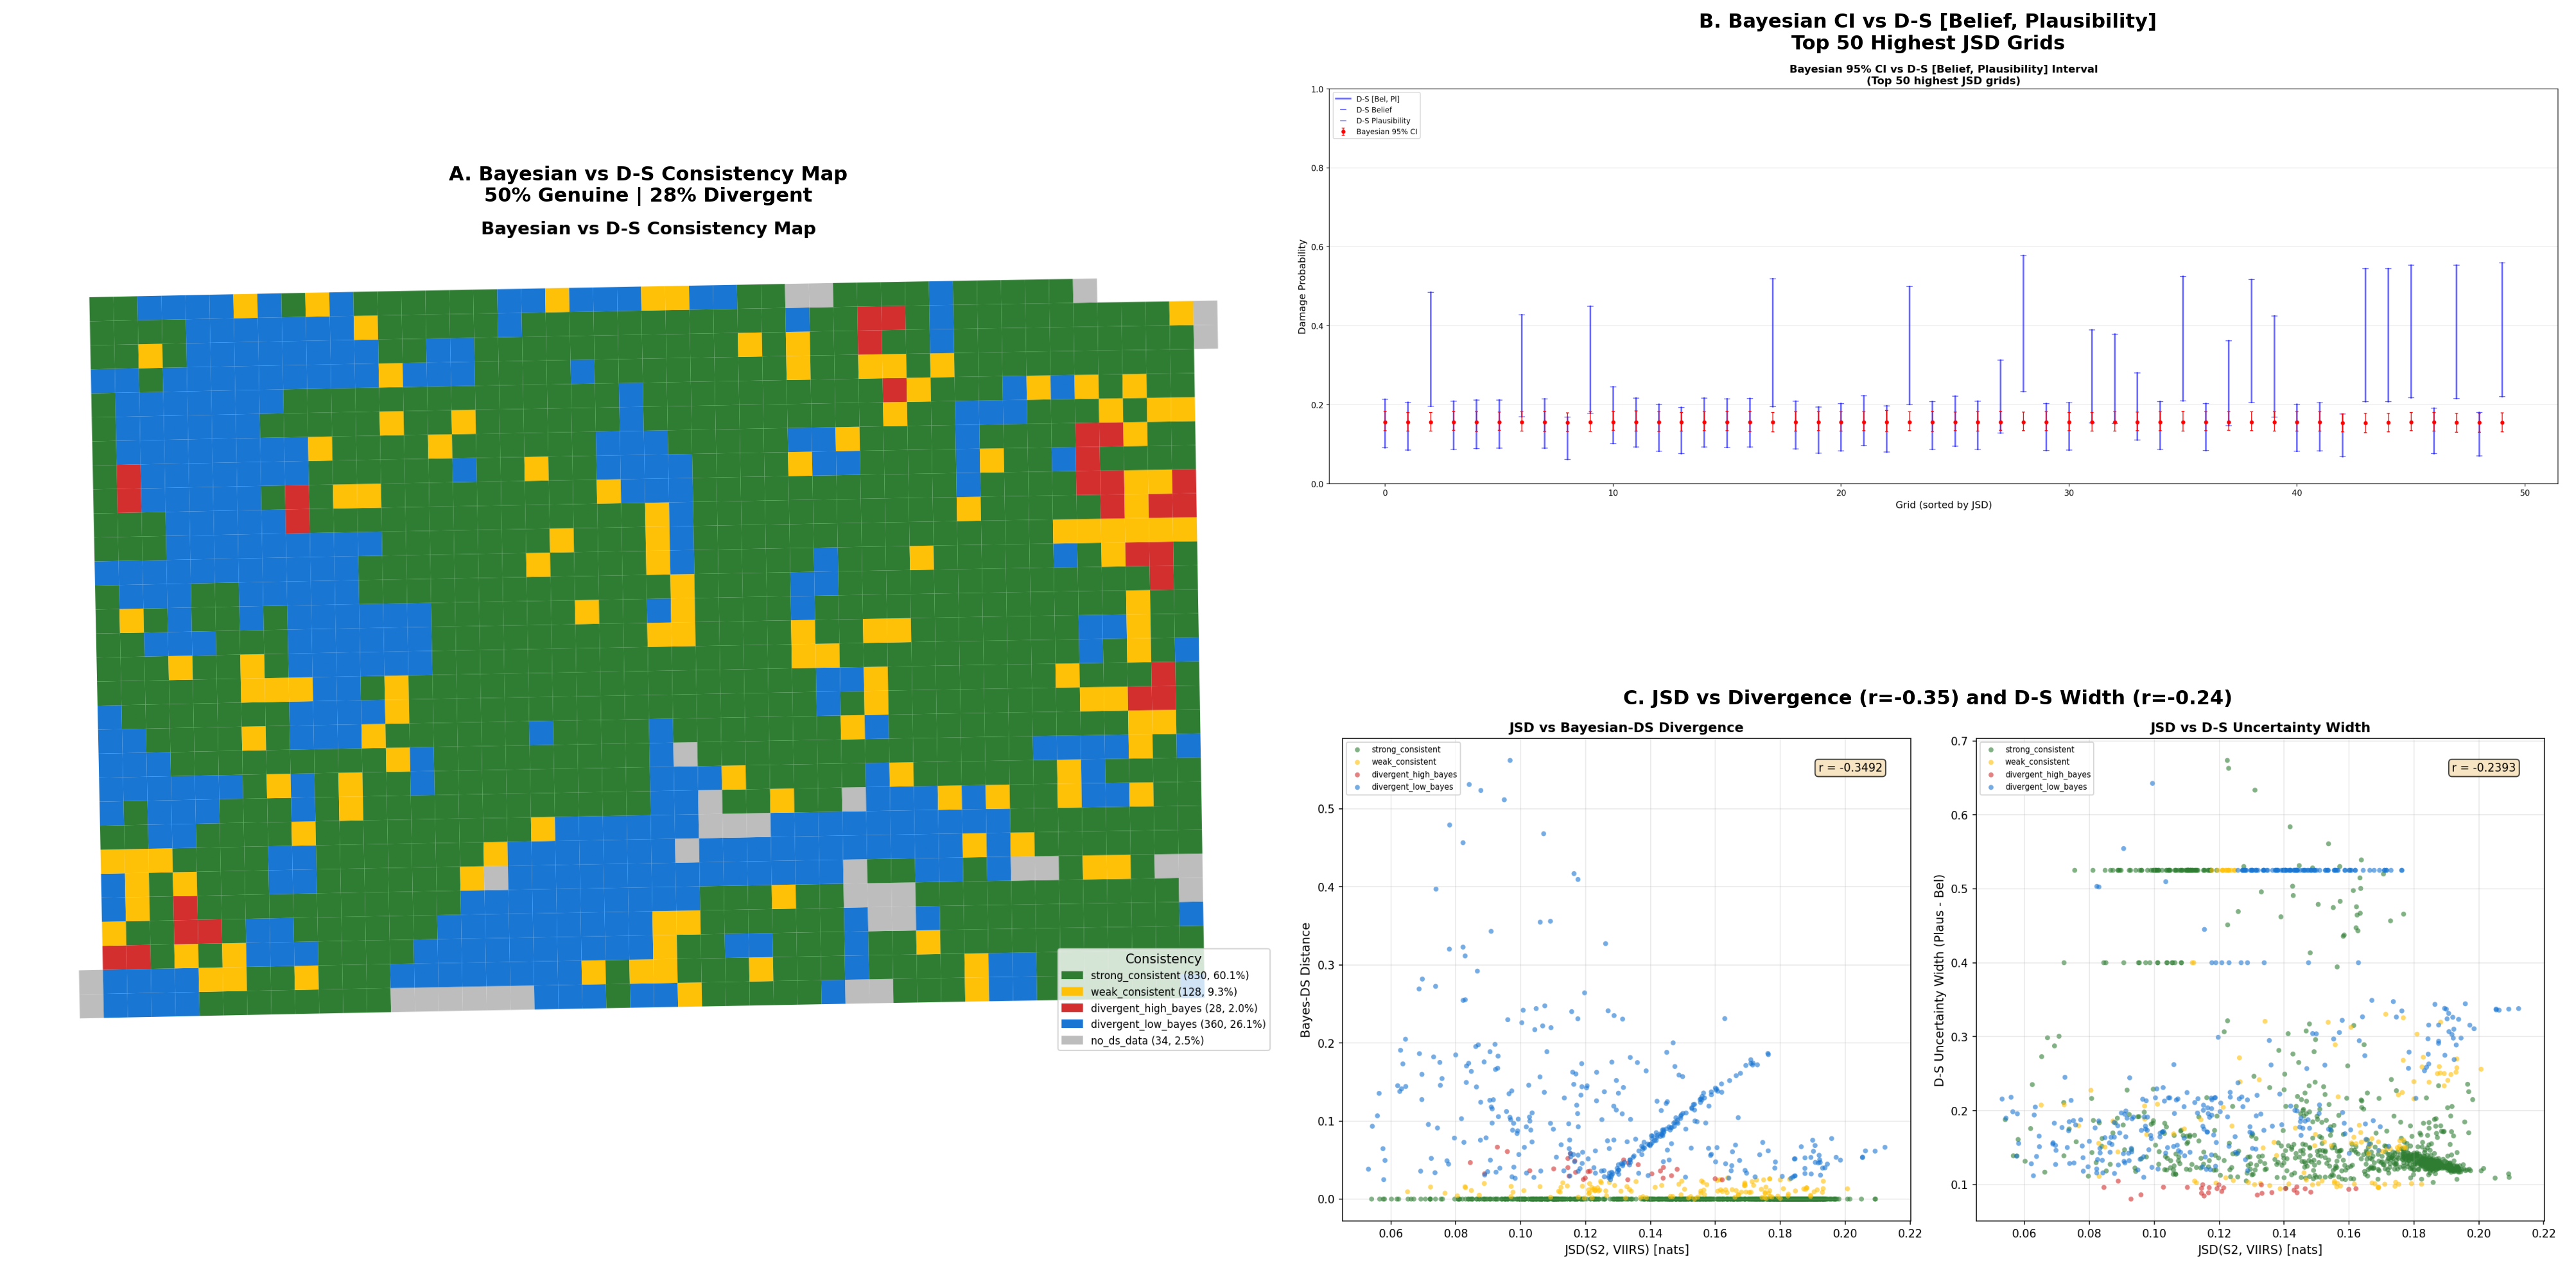
\includegraphics[width=0.95\textwidth]{figures/fig5_bayes_ds_comparison.png}
\caption{\textbf{Bayesian vs.\ Dempster-Shafer under conflicting evidence.}
(A)~Consistency map: $49.9\%$ genuine agreement (green); $10.2\%$
uncertainty-compatible (yellow); $28.1\%$ divergent (red/blue). Divergence
concentrates in the urban core. (B)~Bayesian 95\% CI vs.\ D-S [Belief,
Plausibility] for the 50 highest-JSD grids. D-S intervals (blue) are
consistently wider than Bayesian CIs (red). (C)~JSD vs.\ Bayesian-DS
divergence ($r=-0.35$, left) and JSD vs.\ D-S uncertainty width
($r=-0.24$, right): higher sensor conflict is associated with
\emph{smaller} Bayesian-D-S distance because conflict widens the D-S
interval.}
\label{fig:ds}
\end{center}
\end{figure}

Table~\ref{tab:consistency} and Figure~\ref{fig:ds} provide the grid-level
comparison between the two fusion paradigms. Approximately half of all
grids ($49.9\%$) exhibit genuine agreement: the Bayesian posterior mean
falls within a relatively narrow D-S interval. An additional $10.2\%$ are
classified as uncertainty-compatible, where a wide D-S interval mechanically
covers the Bayesian mean without genuine alignment. The largest divergent
category is ``divergent\_low\_bayes'' ($26.1\%$): the Bayesian posterior
mean ($\approx 0.155$) lies entirely below the D-S belief lower bound.
In these grids, D-S assigns high belief to damage (often driven by strong
single-sensor evidence), while the Bayesian model's hierarchical shrinkage
pulls the estimate toward the population mean. Approximately $60\%$ of
these divergent grids are labeled as undamaged by UNOSAT.

The interval comparison (Panel~B) reveals a structural difference in
uncertainty representation: D-S intervals are consistently wider than
Bayesian credible intervals (mean width $0.225$ vs.\ $0.048$). The
Bayesian model concentrates uncertainty in the hyperparameters and produces
narrow grid-level CIs after shrinkage, while D-S expresses ignorance
through interval width.

A counterintuitive pattern completes the picture (Panel~C): JSD and
Bayesian-DS distance are \emph{negatively} correlated ($r = -0.35$). Grids
with the highest sensor conflict tend to have the \emph{smallest} distance
between the two estimates, because high conflict produces wide D-S
intervals that readily encompass the Bayesian mean. The true divergence
between paradigms is concentrated in grids where sensor evidence is locally
consistent but the Bayesian model's global shrinkage pulls the estimate
away from the D-S interval.

% =====================================================================
\section{Discussion}\label{sec:discussion}

\subsection{Sensor Conflict Is Not Sensor Failure}

The S2 and VIIRS damage indices disagree systematically because they
respond to different physical manifestations of conflict damage. S2
spectral change detects surface alteration---exposed rubble, soil
disturbance, vegetation removal---that may or may not correspond to
building destruction. VIIRS NTL loss detects reduced human activity, which
can arise from structural damage, power grid failure, or population
displacement. A structurally intact but unlit building and a demolished
building near a functioning streetlight produce opposite sensor
signatures---these are not measurement errors but genuine physical
phenomena.

The JSD analysis confirms that every grid exhibits non-negligible sensor
conflict. We therefore caution against interpreting the UNOSAT validation
results as evidence of sensor superiority. Rather, VIIRS shows stronger
agreement with the UNOSAT reference labels under this specific validation
setting, and the current S2-derived index may be more sensitive to a
different damage dimension not captured by the UNOSAT classification
scheme.

\subsection{The Single Latent State Assumption Is Too Strong}

Under the single latent state assumption, the Bayesian model's response to
systematic disagreement is rational: increase uncertainty and shrink toward
the prior. The resulting posterior is internally coherent but limited for
spatial discrimination, producing $p_i \approx 0.155$ for every grid. The
small $\tau=0.063$ and the near-zero KL(Both $\|$ Both$_{\text{global}}$)
are not model failures; they are the logically correct outcome under an
assumption that is violated by the data. The sensor-only baselines
demonstrate that this is not because individual sensors lack spatial
information, but because their spatial patterns are inconsistent with a
shared latent state.

\subsection{Multi-Sensor Fusion Requires Compatible Latent Dimensions}

The fusion suppression ratio of $46.8\%$ provides a quantitative answer to
our third research question: adding a conflicting sensor does not improve
information gain; it actively suppresses usable information. This does not
mean multi-sensor fusion is undesirable---it identifies the necessary
condition: sensors must measure compatible dimensions of the target
phenomenon, or the model must explicitly accommodate multiple latent
dimensions. In the present case, S2 and VIIRS are better understood as
measuring two distinct but correlated damage dimensions---structural
alteration and functional cessation---rather than as noisy replicates of a
single damage state.

\subsection{Toward a Multi-Dimensional Latent Damage Model}

The contrast between Bayesian and D-S paradigms clarifies the trade-off
(Figure~\ref{fig:concept}). The Bayesian model provides a single coherent
posterior but sacrifices spatial discrimination when evidence conflicts.
D-S preserves uncertainty through wider intervals but may over-weight
strong single-sensor evidence in the absence of hierarchical shrinkage.
Neither approach is universally superior. A natural extension is a
multi-dimensional latent damage model with explicitly correlated structural
and functional damage states, where each sensor primarily informs its
corresponding dimension and a correlation structure allows information
sharing. This would preserve the spatial information present in each
individual sensor while still leveraging the benefits of multi-source
fusion.

\begin{figure}[htp]
\begin{center}
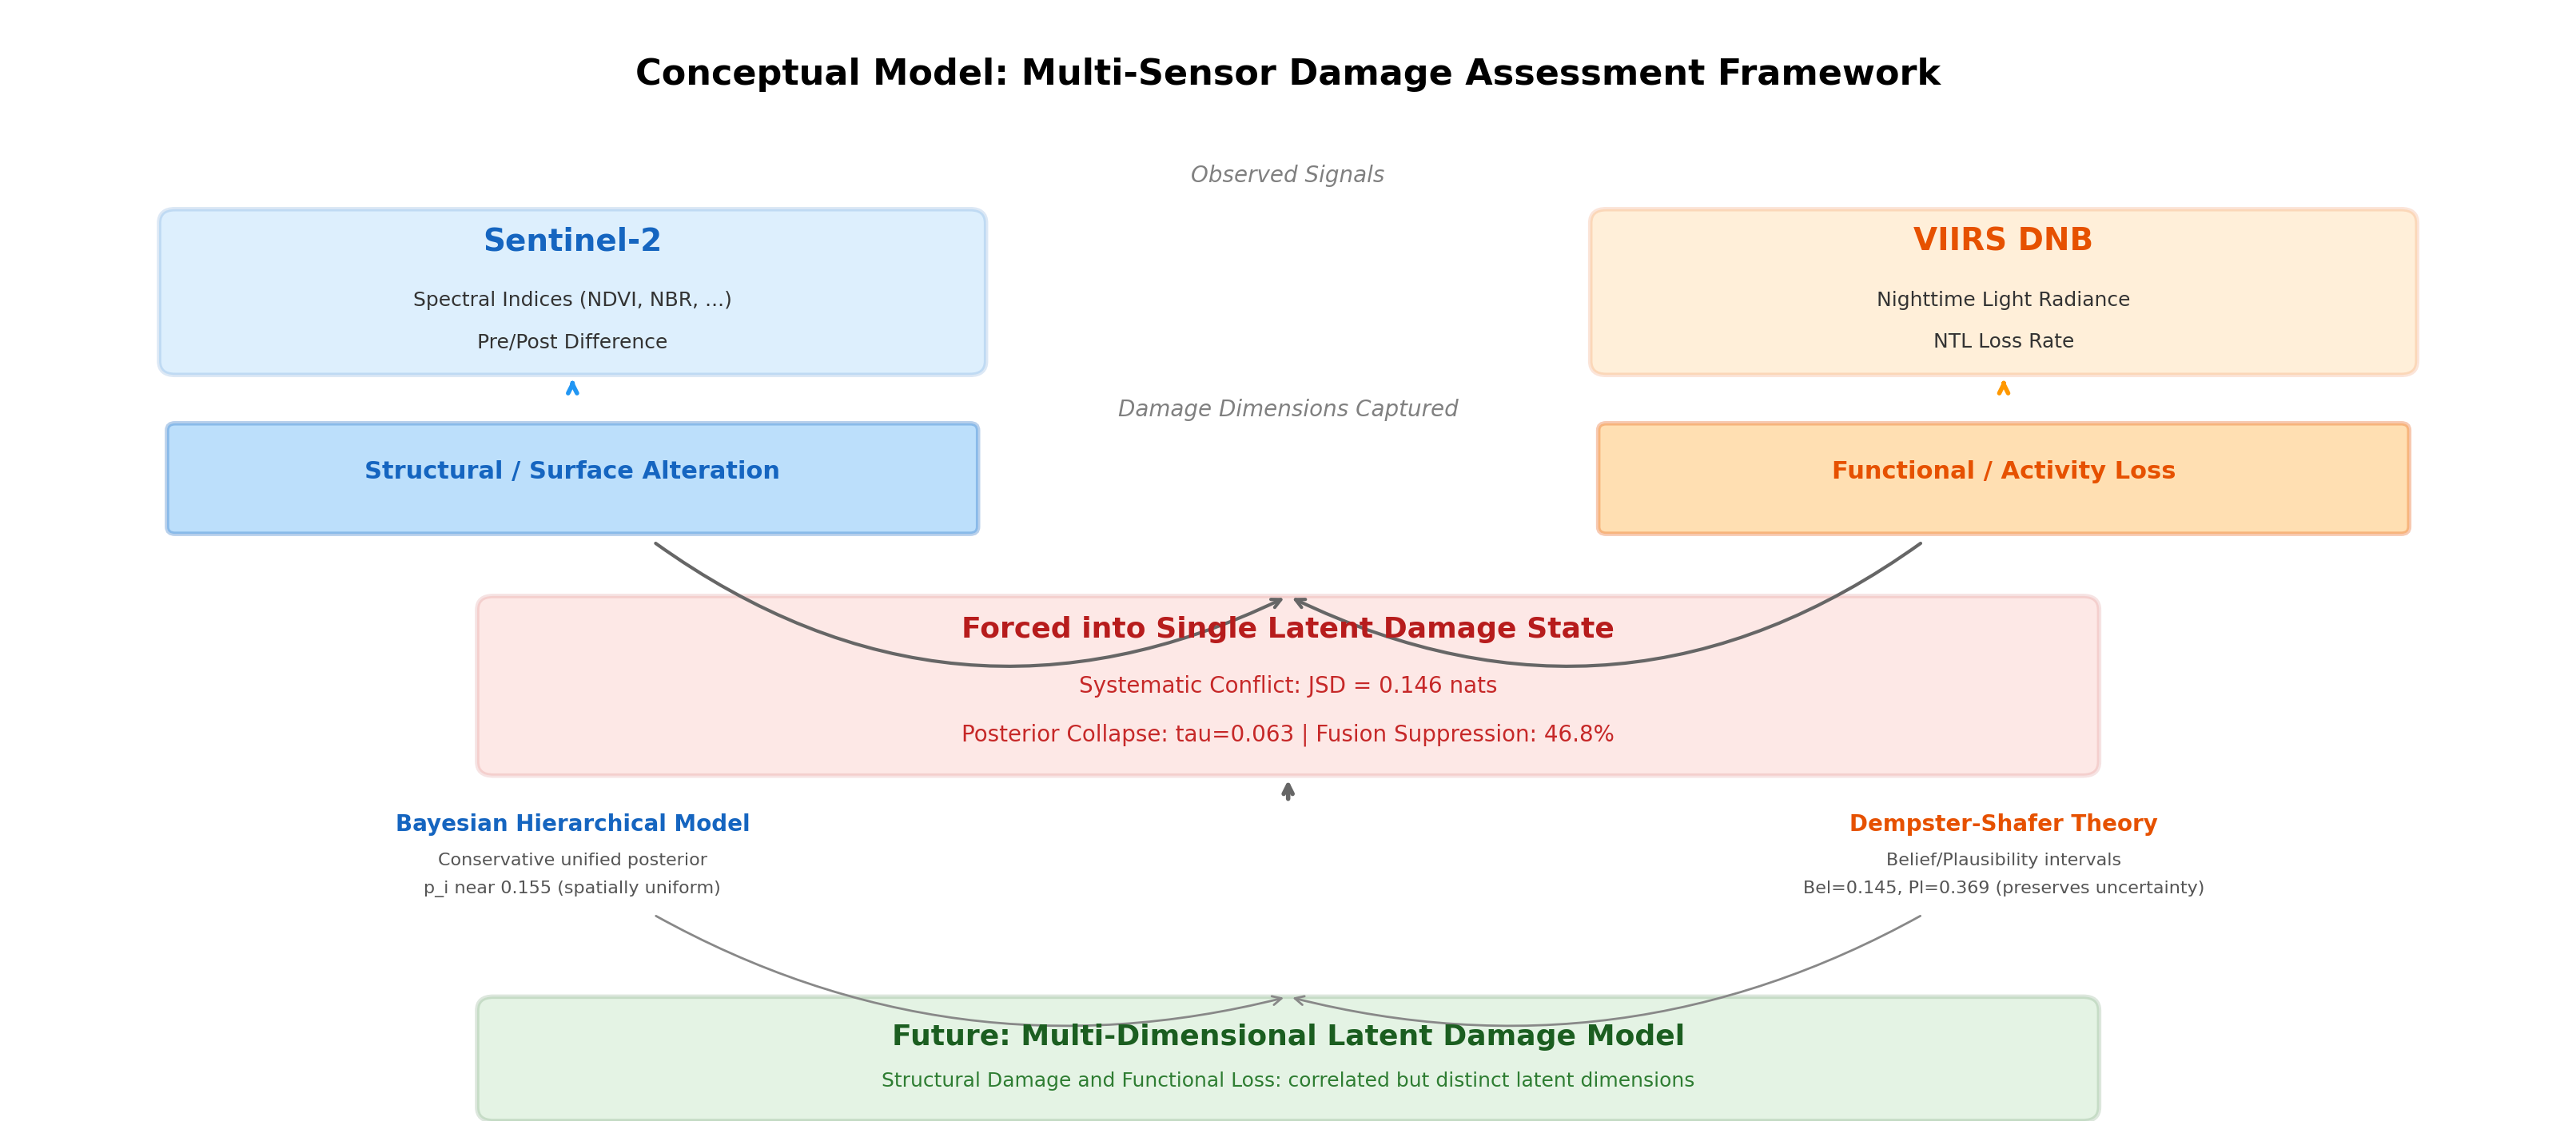
\includegraphics[width=0.95\textwidth]{figures/fig6_conceptual_model.png}
\caption{\textbf{Conceptual model: from single latent state to
multi-dimensional damage assessment.} S2 captures structural/surface
alteration; VIIRS captures functional/activity loss. Forcing both into a
single latent state produces systematic conflict (JSD~$=0.146$ nats),
posterior collapse ($\tau=0.063$), and fusion suppression ($46.8\%$). The
Bayesian hierarchical model yields a conservative unified posterior;
D-S preserves uncertainty intervals. Future work should model structural
and functional damage as correlated but distinct latent dimensions.}
\label{fig:concept}
\end{center}
\end{figure}

% =====================================================================
\section{Limitations}\label{sec:limitations}

\begin{enumerate}
  \item \textbf{UNOSAT is an external reference, not absolute ground truth.}
    It captures visually identifiable building damage but may miss
    functional damage, sub-detection-threshold structural alteration, or
    damage types outside its classification scheme.
  \item \textbf{Single-sensor MCMC diagnostics were weaker than the joint
    model.} The S2-only and VIIRS-only Bayesian models showed elevated
    divergences and $\hat{R}$ values; their posterior ranges should be
    interpreted as diagnostic comparisons rather than precise
    single-sensor uncertainty estimates.
  \item \textbf{Results are conditional on the 500~m grid scale.} Different
    spatial resolutions would yield different conflict and information gain
    estimates due to aggregation effects.
  \item \textbf{Temporal mismatch.} The S2 and VIIRS pre/post pairs capture
    slightly different time windows, and damage processes evolve between
    acquisition dates.
  \item \textbf{The current S2 index is one of many possible formulations.}
    Alternative spectral indices, change detection algorithms, or
    texture-based features could produce different alignment with UNOSAT
    labels.
  \item \textbf{VIIRS NTL loss conflates multiple processes.} Reduced NTL
    can reflect building destruction, power grid damage, population
    displacement, or deliberate blackouts.
  \item \textbf{Single latent state model oversimplifies damage.} Structural
    damage and functional loss are distinct phenomena that a
    multi-dimensional model could better represent.
\end{enumerate}

% =====================================================================
\section{Conclusion}\label{sec:conclusion}

This study examined the fusion of Sentinel-2 spectral indices and VIIRS
nighttime light loss for damage assessment in Mariupol through three
complementary frameworks. Our findings form a coherent evidence chain:

\textbf{Evidence A:} S2 and VIIRS provide non-equivalent damage signals.
The S2-derived index captures structural surface alteration; the VIIRS NTL
loss index captures functional activity cessation. The two scores are
negatively correlated ($r = -0.33$), reflecting their sensitivity to
different physical processes rather than measurement noise.

\textbf{Evidence B:} Under this validation setting, VIIRS shows stronger
agreement with UNOSAT reference labels (AUC~$=0.829$) than the current
S2-derived index (AUC~$=0.332$). All fusion-based scores perform below
VIIRS alone, indicating that combining weakly aligned signals degrades
discriminative performance under single-score aggregation.

\textbf{Evidence C1:} The Bayesian hierarchical model with a single latent
damage state produces a near-uniform posterior ($p_i \in [0.151, 0.157]$,
$\tau=0.063$). Each sensor alone retains spatial structure (S2-only range:
22 pp; VIIRS-only range: 21 pp); the collapse occurs only when both are
forced into a shared latent state.

\textbf{Evidence C2:} KLD/JSD analysis demonstrates that spatial information
is not absent but actively suppressed by conflicting evidence. The fusion
suppression ratio of $46.8\%$ quantifies the information loss, and JSD
$>0.05$ nats across all grids confirms that sensor disagreement is
systematic rather than localized.

\textbf{Evidence C3:} Bayesian and D-S fusion paradigms diverge under
conflict: $49.9\%$ of grids show genuine agreement, $10.2\%$ are
uncertainty-compatible, and $28.1\%$ are divergent. The negative
correlation between JSD and Bayesian-DS distance ($r = -0.35$) reveals that
the two paradigms converge under high conflict (wide D-S intervals encompass
the Bayesian mean) and diverge under locally consistent but globally
conflicting evidence.

\textbf{Conclusion D:} Adding sensors does not automatically improve damage
estimation accuracy. Multi-sensor fusion benefits inference only when the
added sensors measure compatible damage dimensions, or when the model
explicitly accommodates multiple latent states. For conflict damage
assessment, we recommend moving beyond single latent state models toward
multi-dimensional frameworks that distinguish structural and functional
damage as correlated but distinct phenomena (Figure~\ref{fig:concept}).

% =====================================================================
%\acks{This work was supported by...}

\bibliography{references}

% =====================================================================
\appendix

\section{Supplementary Table}\label{apd:tables}

\begin{table}[htp]
\centering
\caption{Method comparison and interpretation.}
\label{tab:methods}
\begin{tabular}{@{}lp{4.5cm}p{5.5cm}@{}}
\toprule
\textbf{Method} & \textbf{What it provides} &
  \textbf{Key finding} \\
\midrule
S2 spectral index &
  Pixel-level surface change score &
  Detects surface alterations; weakly correlated with UNOSAT labels
  (AUC~$=0.33$) \\
VIIRS NTL-loss index &
  Grid-level functional loss score &
  Shows stronger agreement with UNOSAT (AUC~$=0.83$); may conflate
  structural and functional loss \\
UNOSAT validation &
  External reference from visual interpretation &
  Structured benchmark, but itself an imperfect visual-only product \\
Bayesian hierarchical model &
  Unified posterior $p_i$ with 95\% CI &
  Reveals S2-VIIRS irreconcilability; posterior shrinks to mean
  ($p_i \approx 0.155$) \\
KLD/JSD analysis &
  Quantitative information gain and conflict per grid &
  Fusion suppression $46.8\%$; JSD $>0.05$ everywhere proves conflict is
  systematic \\
D-S evidence theory &
  Belief/Plausibility interval without forced convergence &
  Preserves uncertainty (Bel~$=0.145$, Pl~$=0.369$); may over-weight
  strong single-sensor evidence \\
Bayesian vs.\ D-S &
  Grid-level comparison of two paradigms &
  $49.9\%$ genuine agreement; $28.1\%$ divergent; divergence reflects
  tension between shrinkage and evidence weighting \\
\bottomrule
\end{tabular}
\end{table}

\end{document}
